For each independent variable $x_i$ a propagation queue $q_i$ is made. A propagation queue $q_i$ is an 
topological sorting of invariants that are reachable from the vertex representing $x_i$ in the dependency directed 
graph $G$. The vertices in the propagation queue are ordered according to their time stamp in decreasing 
order which is a topological sorting such that there is no backward pointing arc. \\
The propagation queue $q_i$ is used such that each invariant dependent on the value of $x_i$ is updated at most once if 
the variable changes value. The DDG represents which invariant that are directly affected by a change in variable $x_i$ 
but not the order in which they should be updated. Figure \ref{fig_propqueue} shows the necessity of such an ordering. 
\\
\begin{figure}[b]
\centering
\begin{tikzpicture}[scale=1]
        \vertex[label=$x_1$](x1) at (0,2) {};
        \vertex[label=$y_2$](i2) at (2,1) {};
        \vertex[label=$y_1$](i1) at (4,2) {};
        %\vertex[label=$y_3$](i3) at (5,1) {};
         %\vertex[label=$c_2$](c2) at (5,0) {};
    \tikzset{EdgeStyle/.style={->}}
        \Edge(x1)(i1)
        \Edge(x1)(i2)
        \Edge(i2)(i1)
        %\Edge(x1)(c3)
        %\Edge(y1)(c3)
        %\Edge(y2)(c3)
\end{tikzpicture}  \caption{Importance of propagation queue} \label{fig_propqueue}
\end{figure} 
If $y_1$ is updated before $y_2$ then it might need to be updated again after $y_2$ is updated hence updated 
twice. In worst case the number of updates performed when updating $x_i$ could be exponential in the number of vertices 
reachable from $x_i$ instead of linear. \\ 
Once the dependency directed graph is a DAG each invariant vertex has been given a time stamp by Tarjans algorithm. 
Propagation queues are implemented as red-black trees without duplicates hence they have insert time complexity 
$O(log(n))$. For each variable vertex $v_i$ in dependency digraph $G$ a depth first search is made. Each vertex 
visited is added to the propagation queue of $v_i$. This gives a time complexity of $O(rlog(r))$ where $r$ is the 
number of reachable vertices from $v_i$.  \medskip \\ 
During local search when a single variable $x_i$ changes value the change propagate through the DDG using 
the ordering from the propagation queue $q_i$. When two or more variable change value the propagation queues can be 
merged into a single queue removing duplicates.  